\chapter{Experiments and Results}
\label{chap:experiments}

% TODO maybe get rid of this section
\section{Problem Statement}
\label{sec:problem_statement}

In the Deep Q-Network section (\ref{sec:dqn})
I described an approach to deep reinforcement learning.
While the approach works well,
it has not managed to beat all games under consideration
nor would it generalize well to just any game
that fits the input description.
Much care has been taken to make DQN as generic as possible,
yet one detail stands out.

A single state consists of four consecutive image frames
in order to make the problem more Markovian,
a useful trait because it allows us to rely on
useful theoretical properties that have been established
for Markov settings.
However, not all games carry sufficient information
in the last four frames alone.
Some need a few more,
while others could conceivably
show information
that will then be needed to act correctly
after a long period of time has passed.
In other words, there could be hidden state
that the agent nevertheless had access to
at some point in the past.

\paragraph{}
My goal is now to explore different approaches
to this fixed-window history approach,
to explore different ways of dealing with time.
Ideally,
the learning technique should not employ an approach
that contains a fixed window anywhere at all.
However, such techniques are considered here as well.
% TODO discuss POMDP

\paragraph{}
The rest of this chapter is organized as follows.
First, I will examine the Arcade Learning Environment
in close detail in so far as this benefits
the following sections.
Then, I will closely investigate three approaches
to the time problem.
The three techniques discussed in this thesis are
\textit{Late Fusion},
\textit{3D Convolutions}
and \textit{LSTMs}.
Each in turn will be discussed,
then explored and evaluted.
Finally,
I will draw the conclusions of this thesis
in \ref{sec:conclusions}.

\section{Arcade Learning Environment}
\label{sec:arcade_learning_environment}
In order to fully understand the experiments that follow
and the implications of their results,
it is important to first have a closer
look at the Arcade Learning Environment
\parencite{bellemare13arcade}.
ALE is built on top of Stella
\footnote{http://stella.sourceforge.net},
an open-source Atari emulator.
It enables one to programmatically interact
with any compatible Atari game file.
This includes getting the screen in raw pixels,
access to the Atari's emulated RAM,
the game's current score
and actually interacting with the game by sending actions.

\paragraph{}
To appreciate the setting completely we will need to
investigate the hardware the games considered here used to run on.
The Atari 2600 was released in 1977.
Its CPU ran at 1.19 Mhz,
more than a 1000 times slower
than a single average core used for personal computers nowadays.
The size of the RAM was especially small compared to
what is used in modern days, with 128 bytes.

Of special interest to us is the console's graphic component.
The screen is 210 by 160 pixels
and could display up to 128 colors.

The Atari 2600 console is interacted with using
a joystick and a button.
The joystick can move in 8 directions.
Combining that,
along with pushing the button
while moving the joystick
(or not moving it)
gets us to 17 distinguishable actions.
Add one for not doing anything at all
and we have a total of 18 actions for our learning agent.

% TODO consider getting rid of this,
% just thought it was nice to see wtf it is
\begin{figure}[h]
\center
\begin{subfigure}[t]{.5\textwidth}
  \centering
  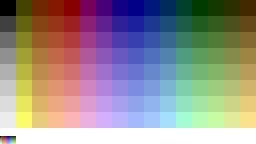
\includegraphics[width=\textwidth]{ntsc_palette.png}
  \vspace{.1\baselineskip}
  \caption{
    The Atari 2600 NTSC Palette used by many games.
    It allows 3 bytes for luminiscence
    and 4 bytes for chrominance,
    resulting in the 128 distinct colors
    you see here.
  }
  \label{fig:nips_network}
\end{subfigure}
\hfill
\begin{subfigure}[t]{.4\textwidth}
  \centering
  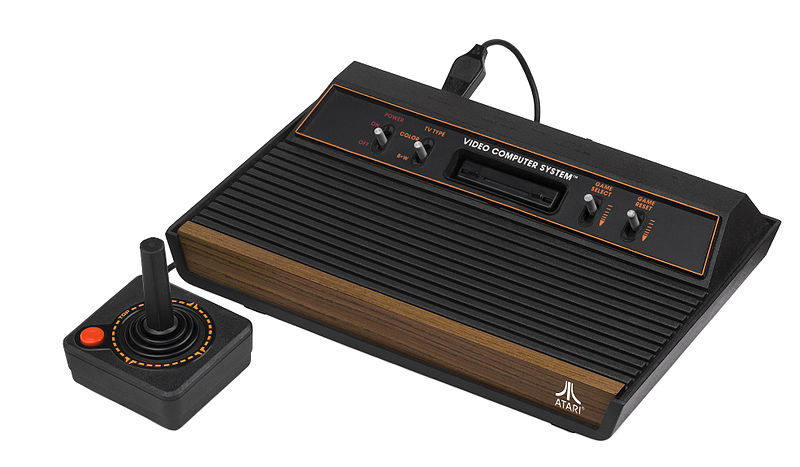
\includegraphics[width=\textwidth]{atari.jpg}
  \vspace{.1\baselineskip}
  \caption{
    The Atari 2600 with its joystick.
  }
  \label{fig:nature_network}
\end{subfigure}
\caption{}
\label{fig:dqn_networks}
\end{figure}

\subsection{Shortcomings}
\label{sub:shortcomings}
While the Atari's computational simplicity,
small screen
and relatively straightforward games
make it a great testbed for reinforcement learning,
the same characteristics
bring along a few shortcomings
that bear discussing.

\paragraph{}
First off, the Atari 2600
is entirely deterministic.
% TODO really want a ref on this
This allows some games to be abused
by learning how to exploit bugs
or otherwise causing situations
that would be very hard for a human to replicate,
yet that a learning algorithm could easily manage
in a deterministic setting.

This exploitation of a game's weak points
does not sound bad on its own
- after all, the agent is learning -
but it is obviously a case of overfitting
which should preferably be avoided.

% TODO should I mention in DQN?
DQN tries to avoid this by adding a random amount
of nullops at the start of the turn,
that is, the agent waits a random amount of turns
before it can play.

\paragraph{}
The console's determinism makes it so
that given the agent's history,
the next state given an action
can be known exactly.
However,
very few games actually need more than
a few frames of history
in order to achieve this Markov property.

Since the main interest of this thesis
is dealing with time,
long-term time dependencies would be especially interesting to investigate.
Sadly, however good of a testing environment ALE may seem,
it lacks thoroughly in this regard.
% TODO erase this if you don't
I will discuss later how to circumvent this lack of complexity partially.

\paragraph{}
% TODO(final) adjust if needed
I will now discuss two games in some detail
and shed light on their core distinctions
in order to later understand and explain
the differences between their learning results.

\subsection{Space Invaders}
\label{sub:space_invaders}

\subsection{Pong}
\label{sub:pong}

\subsection{General Setup}
\label{sub:general_setup}
All experiments that follow will be based on the DQN architecture
devised by \cite{Mnih2013}.


\section{Late Fusion Network Approach}
\label{sec:late_fusion_network_approach}
The first alternative to the standard DQN
considered here is
the Late Fusion DQN architecture
inspired by \citeauthor{Karpathy2014} (\citeyear{Karpathy2014})
who successfully deployed it for
action recognition in video clips.
The base premise for this architecture
is that in order to capture time dependencies
it is sufficient to look at differences
between frames.
Presumably,
this works better with short-term dependencies
as differences between frames close to each other in time
are smaller.

Also, Late Fusion
considers two frames with a fixed distance in time in between.
This can only yield good results for longer time dependencies
if the dependency always spans approximately the same amount of time,
a requirement that is undesirable
and not always satisfiable.

\paragraph{}
The Late Fusion DQN is based on the default DQN implementation.
In fact, the learning algorithm is entirely the same
and parameters are as depicted in Table \ref{tab:base}.

Instead of a single stack of convolutional layers,
we now have two towers that each take as input a single frame.
The frames are separated by a fixed amount of frames
that go unused for the pass.
Each of the two towers has no access to the frame
that is input to the other one.
Rather, the towers get combined by a fully connected layer
that is also the first of the layers that has access
to both time steps.

Since each convolutional network now only has a single frame as input,
we suddenly get back the image channel input dimension (depth)
that was previously used to stack frames together.
In order to use that dimension for time,
DQN uses a grayscale
which only requires a single scalar value
and as such this channel dimension was implicit before.
Now that we have access to an extra input dimension
we can again use color channels
such as RGB,
which might add useful information to the model.

\paragraph{}
The general gist to the Late Fusion architecture
is that the convolutional layers
compute high-level features
which the fully-connected layer can then compare
in order to compute the correct output.

The full architecture is depicted in Figure \ref{fig:late_fusion}.

\begin{figure}[htpb]
  \centering
  % \captionof{figure}{Late Fusion Network}
  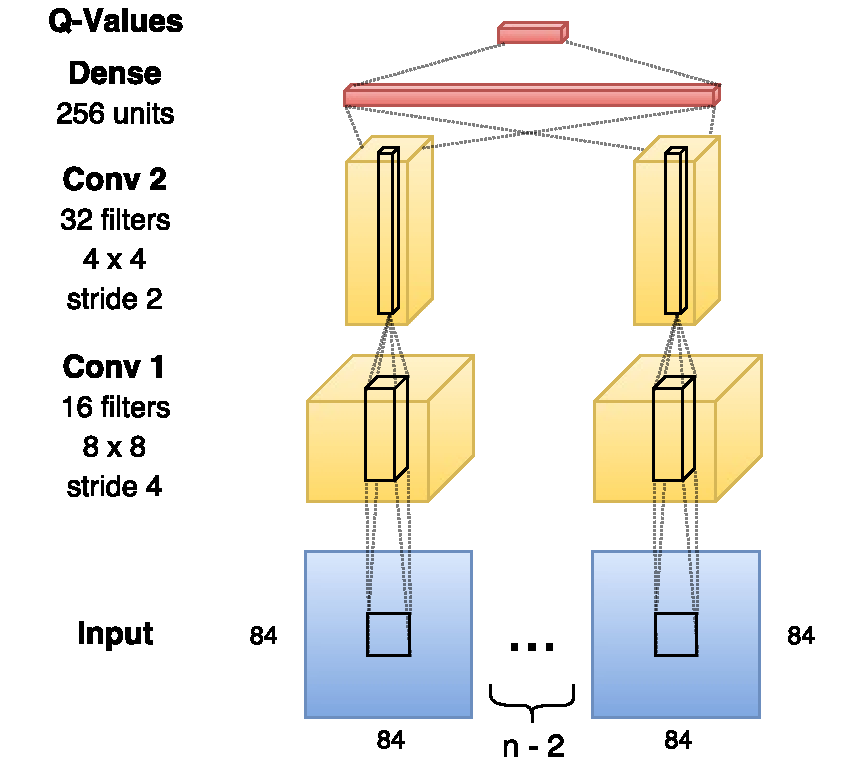
\includegraphics[width=0.8\linewidth]{late_fusion.pdf}
  \caption{
    Late Fusion DQN.
    A sample of $n$ consecutive frames is chosen
    but only the outer two frames
    feed into the network.
    The features learned by the two convolutional networks
    is combined through the fully-connected layer
    that combines both.
    Only from the fully-connected layer up
    is information from two different time steps available.
  }
  \label{fig:late_fusion}
\end{figure}

\subsection{Tuning}
\label{sub:late_fusion_tuning}


\section{3D Convolutional Network Approach}
\label{sec:3d_convolutional_network_approach}
Building on the idea that time is an extra spatial dimension
and should not be handled differently
from image width or height,
I investigate 3D convolutional layers next.
In the original DQN implementation
the time dimension gets flattened immediately
by the first convolutional layer
and is not present explicitly
in its output;
only the first convolutional layer
has explicit access to time
because the 2D convolutional layer implementation
extends along the entire depth of the input.
Intuitively this means that only low-level
features over time can be learned
whereas we can easily imagine
more abstract features
that relate to time.
This is where the 3D convolutional network comes in,
in order to allow us to specify step size and stride across time
in order to control how time is propagated through the entire network.

\paragraph{}
The 3D Convolutional DQN
is again based entirely on the original DQN implementation
\parencite{Mnih2013},
with parameters in table \ref{tab:base}.


\begin{figure}[htpb]
  \centering
  \begin{subfigure}[b]{\textwidth}
    \centering
    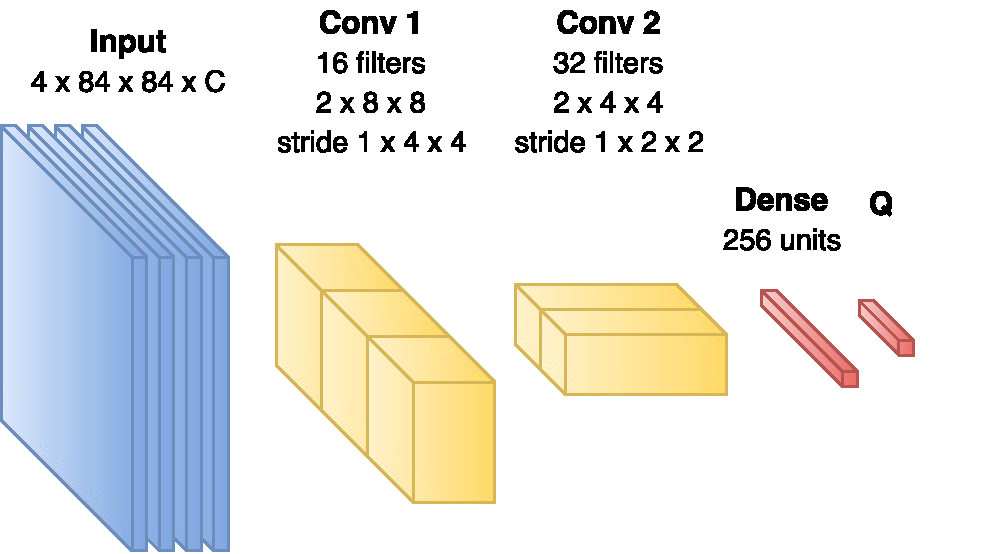
\includegraphics[width=\textwidth]{conv3d_network.pdf}
    % \vspace{.1\baselineskip}
    \caption{
      3D convolutional DQN.
      The input consists of 4 frames
      that can each have $C$ image channels.
      Both convolutional layers employ a time filter size of 2,
      meaning a single weight corresponds to
      two frames of the layer's input.
      Combined with a time stride of 1,
      the time dimension of the output of each consecutive layer
      is 1 smaller than its input.
    }
    \label{fig:conv3d_network}
  \end{subfigure}
  \begin{subfigure}[b]{.30\textwidth}
    \centering
    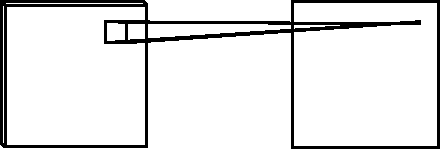
\includegraphics[angle=-90,width=.49\textwidth]{2dconv.pdf}
    \caption{
      2D convolution for a single feature
      for a single frame with multiple channels.
    }
  \end{subfigure}
  \hfill
  \begin{subfigure}[b]{.64\textwidth}
    \centering
    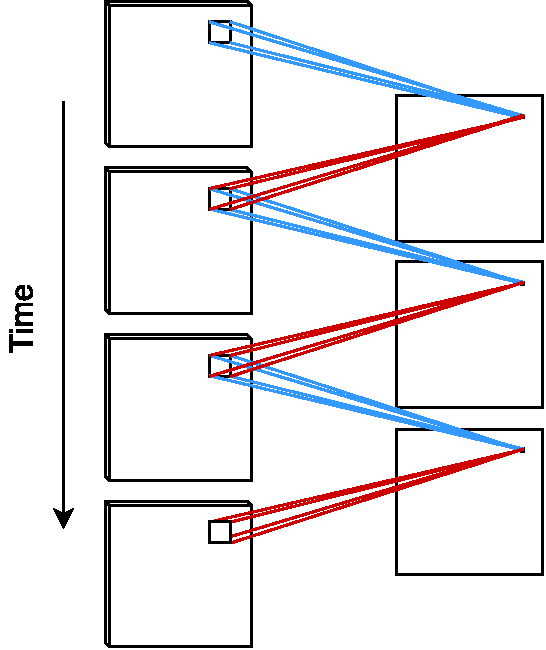
\includegraphics[angle=-90,width=\textwidth]{conv3d_time.pdf}
    % \vspace{.1\baselineskip}
    \caption{
      3D convolution for a single feature
      (depth slice of the convolutional layer)
      with 4 input frames
      and a time filter size of 2.
      Connections of the same color depict shared weights.
    }
    \label{fig:conv3d}
  \end{subfigure}
  \label{fig:conv3d}
\end{figure}

\section{Long Short-Term Memory Approach}
\label{sec:long_short_term_memory_approach}



\section{Conclusions}
\label{sec:conclusions}


